\documentclass[paper=a4, fontsize=11pt]{scrartcl}
\usepackage[T1]{fontenc}
\usepackage{fourier} 
\usepackage[english]{babel} 
\usepackage{amsmath,amsfonts,amsthm} 
\newtheorem{theorem}{Theorem}
\theoremstyle{definition}
\newtheorem{definition}{Definition}[section]
\usepackage{mathtools}
\DeclarePairedDelimiter\ceil{\lceil}{\rceil}
\DeclarePairedDelimiter\floor{\lfloor}{\rfloor}
\usepackage[ruled,vlined]{algorithm2e}
\usepackage{float}
\usepackage{hyperref}
\usepackage{sectsty} 
\allsectionsfont{\centering \normalfont\scshape} 
\usepackage{fancyhdr} 
\pagestyle{fancyplain}
\fancyhead{}
\fancyfoot[L]{}
\fancyfoot[C]{}
\fancyfoot[R]{\thepage}
\renewcommand{\headrulewidth}{0pt}
\renewcommand{\footrulewidth}{0pt}
\setlength{\headheight}{13.6pt}
\setlength{\parskip}{0.5\baselineskip}
\numberwithin{equation}{section}
\numberwithin{figure}{section} 
\numberwithin{table}{section}
\setlength\parindent{0pt}
\usepackage{xcolor}
\usepackage{graphicx}
\definecolor{linkcolor}{HTML}{00008B}
\definecolor{shade}{HTML}{D4D7FE}
\definecolor{text1}{HTML}{000000}
\definecolor{headings}{HTML}{00008B}
\hypersetup{colorlinks,breaklinks,
            urlcolor=linkcolor,
            linkcolor=linkcolor
}
\usepackage{listings}
\lstset{
  basicstyle={\small\ttfamily},
  keywordstyle={\bfseries\color{NavyBlue}},
  breaklines=true,
  emphstyle={\bfseries\color{Rhodamine}},
  commentstyle={\color{PineGreen!60!black}},
  stringstyle={\rmfamily\color{YellowOrange}},
  showstringspaces=false,
  frame=shadowbox,
  breakatwhitespace=false,
  captionpos=b,
  extendedchars=true,
  keepspaces=true,
  numbers=left,
  numberstyle=\tiny,
  rulecolor=\color{black},
  rulesepcolor={\color{blue!20!white}},
  showspaces=false,
}
\newcommand{\horrule}[1]{\rule{\linewidth}{#1}}

% TODO: comment here after finished
\usepackage{draftwatermark}
\SetWatermarkText{DRAFT}
\SetWatermarkScale{1}

\title{	
\normalfont \normalsize 
\textsc{Final Team Report for ``Human Computation'', Summer Term 2017, IFI LMU} \\ [25pt]
\horrule{0.5pt} \\[0.4cm]
\huge Final Team Report for HC System: \\
A Novel GWAPs Disaster Monitoring System\\
\horrule{2pt} \\[0.5cm] % Thick bottom horizontal rule
}
\author{
  \\ Team: Hotpot\\
  Changkun Ou : <11406972> \\
  Yifei Zhan : <11462563> \\
  Zhe Li : <11194275>  }
\date{\today}

\begin{document}
\maketitle
\tableofcontents

\paragraph{Abstract}
Disaster Monitoring is a challanging problem due to the lack of infrastructures in the control area.
This report contributes to a Game With A Purposes (GWAPs) based human computation system, 
which analyzes tagging results from players for satellite pictures and exports aggregated results to stakeholders. 
We illustrated our system prototype and implementation technology stack, as well as the mathematical model of the scheme. 
As justification and evaluation, we proved the correctness of the model, 
discussed issues caused by this system and possible solutions, extensions for future works.

\section{Introduction}

In this chapter, we will give an introduction about the backgrounds of UNICEF and the related technics 
used in the project. The simple definition of HC system and GWAPs will be given. 
The purpose of our HC system and the contribution of human beings will also be talked.

\subsection{Related Works}

\subsubsection{UNICEF}
The United Nations Children's Fund \cite{unicef1994state} is a United Nations programme headquartered
in New York City that provides humanitarian and developmental assistance to 
children and mothers in developing countries \cite{wiki:UNICEF}.
It works in 190 countries and territories to protect the rights of every child. 
UNICEF has spent 70 years working to improve the lives of children and their families. 
Defending children's rights throughout their lives requires a global presence, 
aiming to produce results and understand their effects. 
In Syrian, the UNICEF works on providing and transporting critical medicine, 
aid and supplies to the refugees living in the war areas. The challenges UNICEF meet is that 
there are many hard-to-reach (HTR) and besieged (BSG) areas and the supplies are 
very hard to be delivered to these zones if the UNICEF have no idea about 
the real time war situation and the disaster level. It will cost too much for the UNICEF 
which is just a Non-profit organization if they entirely hire employees to 
collect the data of war situation. 
Our work is to design and develop a Human Computation system by GWAP \cite{lafourcade2015games}.

\subsubsection{HC System and GWAPs}
Human Computation system is a paradigm for utilizing the human processing power to solve problems that 
computers cannot yet solve \cite{quinn2011human}. 
It is the system of computers and large numbers of humans that work together in order to solve problems that 
could not be solved by either computers or humans alone \cite{quinn2009taxonomy}.
Our HC system is a kind of GWAPs, which uses enjoyment as the primary means of motivating participants. 
One of the challenges in any human computation system is finding a way to motivate people 
to participate \cite{quinn2011human}. 
Besides the enjoyment, we will design some interactions between users and our system to 
make the volunteer users feel honored for their contribution.

\subsection{Purpose of the System}
The users are required to select a \textbf{Region Of Interests(ROI)} upon the presented satellite images 
and tag the ROI from a provided tag list or input their own tag. Anyone can directly participant 
without registration, but the system will record an ID of each user.
Computer Graphics can also be a way to detect and recognize the map images, but it will cost 
too much time and money in developing recognition algorithms and the best 
computer graphics algorithm currently can not beat the image recognition ability of human beings. 
That's the reason we design the HC system to solve the problem.

\subsection{Human contribution to the System}
The Computer Graphic techniques and Artificial Intelligence grow very fast in recent years, 
however, it is still a great problem for computers to detect and recognize images accurately and fast.
Nevertheless, it is a simple thing for human beings to do it.
The HC system for disaster monitoring encourages more Internet users to contribute information 
to solve the image tagging problem by GWAPs. 
We developed the Player Rating Model to guarantee the quality of collected information 
and some interesting feedback and interaction are designed to maintain the enjoyment of players in the game.
Users do some image tagging tasks in the game by their computing power and intelligent 
which are contributed to collect data in the map images.


\section{Functionality of a novel HC system}
  \subsection{Functionality as seen by a user}

%   user workflow

    A player can finish infinity Round tasks, 
    a Round task contains {N} tagging tasks, 
    the player tagging task is to:

    \begin{itemize}
      \item Select a Region Of Interests(ROI) upon the presented satellite image;
      \item Tag the ROI from a provided tag list or input their own tag, the provided tag list contains: $T_1, T_2, …, T_n, \text{other(input needed)}$
    \end{itemize}

    Note that:

    \begin{itemize}
      \item A ROI is a sub-rectangle-window of a image;
      \item Multiple selections;
      \item Anyone can directly participant without registration, but system records an ID
    \end{itemize}

  \subsection{Functionality as seen by a stakeholder}
  \subsection{Incentivization concept}

      \subsubsection{Task Generator}

    A task generator combines images from satellite and Result DB:

    \begin{itemize}
      \item Split a certain monitoring area image to pieces of images;
      \item Mix images from Result DB and pack as a Tagging Task which to be assigned to player.
    \end{itemize}

    \subsubsection{Player Rating Model}

    Player’s input vector: 
    
    \[
    (\text{anonymous\_id}, \text{image}, \text{event\_time}, \text{ROI}, \text{tag\_list})
    \]

    Model output: 
    
    \[
    (\text{anonymous\_id}, \text{trust\_value})
    \]

    Note that:

    \begin{itemize}
      \item $(anonymous\_id, image, event\_time, ROI)$ is the primary key of the input vector;
      \item A player can generate multiple vectors to rating system even for same image;
      \item The event\_time is the capture time of the satellite image.
    \end{itemize}

    \begin{figure}[htp]
    \centering
    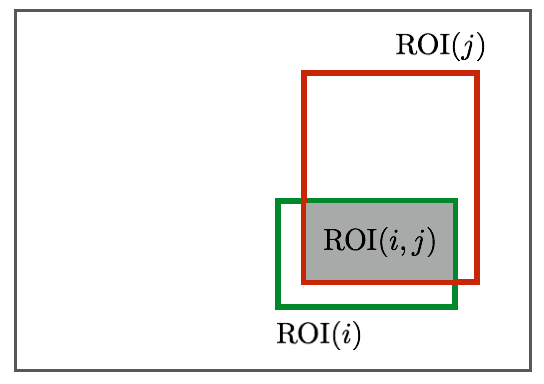
\includegraphics[width=4cm]{figures/weight-define}
    \caption{Weight Definition Visualization}
    \label{fig:roiweight}
    \end{figure}

    For a certain image $img$ at time $t$, Rating: player $i$ $\rightarrow$ player $j$:

    \[
    w_{ij}=\sum_{\text{ROI}\in \text{ROIs}}\frac{\text{ROI}(i,j)}{\text{ROI}(i)} \times \frac{Cov(\text{tags}(i), \text{tags}(j))}{\text{var}(\text{tags}(i))\text{var}(\text{tags}(j))} \geq 0
    \]

    Normalized Adjacency Matrix:

    \[
    A = (\frac{w_{ij}}{\sum_{j}{w_{ij}}})
    \]

    Obviously, A is \textbf{irreducible, real, non-negative, column-stochastic, and diagonal element being positive,} then eigenvalue of A is the player trust value.

    When a new player tagging task need to be rated,

    \begin{itemize}
      \item which means we need introduce a new node to the graph
      \item need calculate the trust value of new graph
      \item let $t’$ is the trust value of new player
      \item if $t’ >= \text{mean}(\text{old\_eigenvalues})$, then it is a reliable player, otherwise drop it.
    \end{itemize}

    \subsubsection{Disaster Level Evaluation Model}

    Query input:

    \[
    (\text{time}) or (\text{area\_id})/(\text{area\_id}, \text{time})
    \]

    Model output:

    \[
    (\text{area\_id}, \text{time}, \text{disaster\_level})
    \]

    Note that:

    \begin{itemize}
      \item All results are evaluated from reliable tasks
      \item Evaluation Model generated by all reliable history
    \end{itemize}

    Now we have trusted results, each area has its tagging history.

    For an area at time t, define disaster level as follows:

    \[
    v_{area} = \frac{
    \sum_{\text{tag}\in\text{tags}}
      {w_{tag}\times\#(\text{tag})}
    }
    {\sum_{area\in areas}{\sum_{\text{tag}\in\text{tags}}{w_{tag}\times\#(\text{tag})}}}
    \]

    where $w_{tag}$ is pre-defined weight by system, $\#(tag)$ is the occur number of a tag.

    Return value:

    \begin{itemize}
      \item disaster region: $\cup_{ROI\in ROIs}{ROI}$
      \item disaster level: $v_{area}$
    \end{itemize}

    \subsubsection{Data Persistence}

    Trusted DB Fields:

    \begin{lstlisting}[
      caption={Trusted Database Field},
      label={lst:trustdb}
    ]
    [
        {
            "anonymous_id": number,
            "tasks": [
                {
                    "image": image_path,
                    "at_time": time, 
                    "ROI": [
                        {
                            "latitude": number,
                            "longitude": number,
                            "tags": [tag1, tag2, ...]
                        }
                    ]
                }
            ]
            "trust_value": number
        }
    ]
    \end{lstlisting}

    Result DB Fields:

    \begin{lstlisting}[
      caption={Results Database Field},
      label={lst:resultdb}
    ]
    [
        {
            “area_id": number,
            "history": [
                {
                    “at_time”: time,
                    "image": image_path,
                    "ROI": [
                        {
                            "latitude": number,
                            “longitude": number,
                            "tags": [tag1, tag2, ...]
                        }
                    ],
                    "disaster_level": number
                }
            ]
        }
    ]
    \end{lstlisting}


\section{Design}

In this chapter, we describe the overall design of our disaster monitoring backend system in details.
Firstly, we propose our system architecture of this disaster monitoring;
Then we specify and justify our most critical system components such as databases design, 
\textbf{Player Task Generator (PTG)\label{idx:ptg}}, \textbf{Player Rating Model (PRM)\label{idx:prm}} 
as well as \textbf{Disaster Evaluation Model (DEM)\label{idx:dem}}.

With these components, model and databases, the disaster monitoring system can handle
common problems in HC system, such as cold start, malicious player detection, etc. 
It is also expandable, portable and can be easily applied to any other same image selection 
and tagging based HC system in different areas.

\subsection{System Architectures}

Figure \ref{fig:arch} illustrate the overall disaster system design.
The system databases are composed of two different type of databases. 
The first database \textbf{PlayerDB} combines \textbf{TrustedDB} and \textbf{UntrustedDB} 
where persistent the player property and raw tagging inputs whether the overall result is reliable or not.
The second database is called \textbf{ResultDB} where persistent the reliable player inputs.

\begin{figure}[htp]
\centering
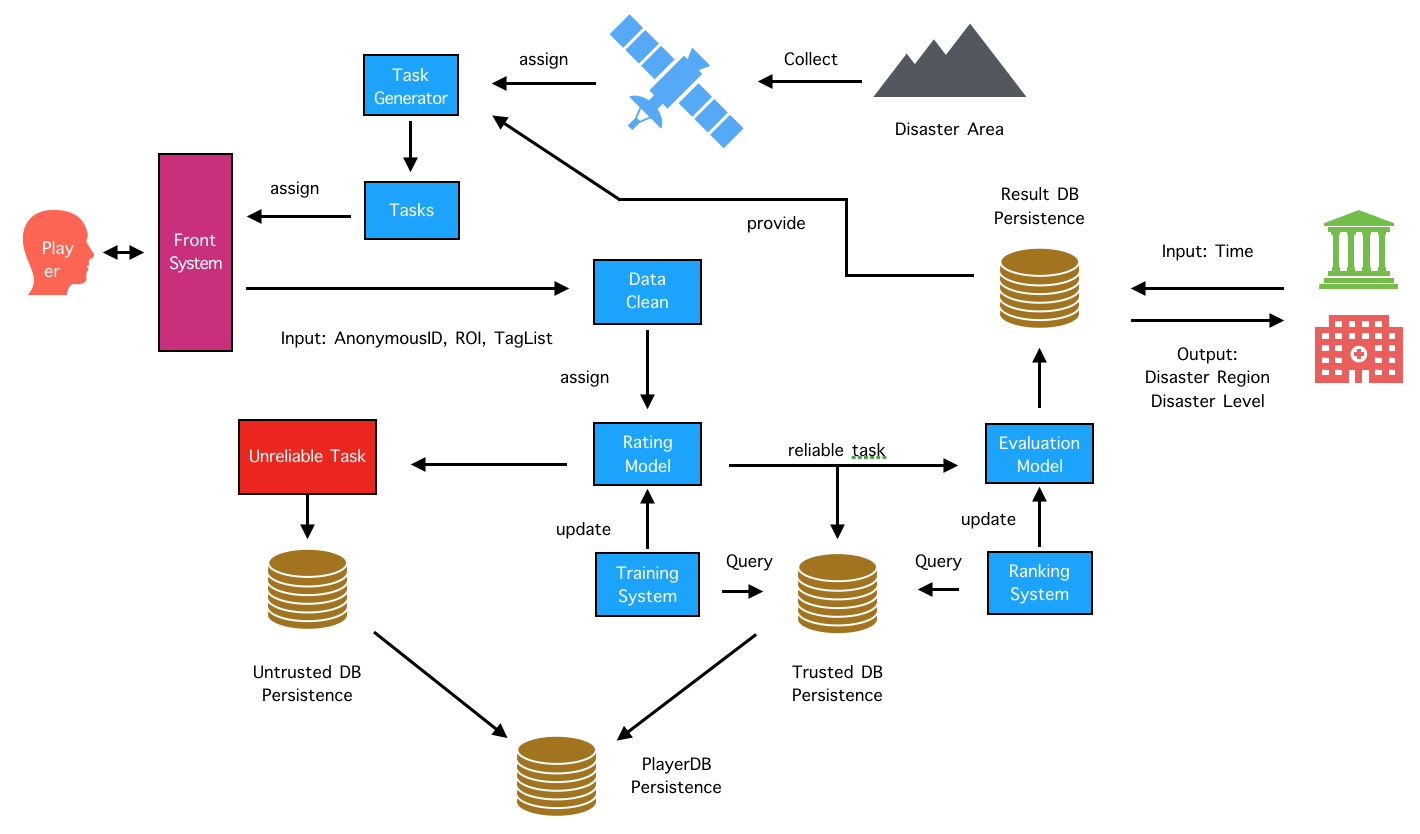
\includegraphics[width=0.9\textwidth]{figures/system2}
\caption{System Design Overview}
\label{fig:arch}
\end{figure}

For this architecture design, one can simplify the overall data flow into tree main steps 
that describes as follows:

\begin{itemize}

\item [Step 1.]  Player task generating: 
We propose the \textbf{\hyperref[idx:ptg]{PTG}}
that combines trusted results from TrustedDB, 
and separate new images from satellite, then assign this binding to the future players.

\item [Step 2.] Malicious player detection: 
A reliable player shall pass the malicious detection algorithm (describe in algorithm \ref{algo:malicious})
inside the \textbf{\hyperref[idx:prm]{PRM}}. 
Once the player is not a malicious player, then system will mark all the results from this player
as a reliable result and then send it into next step.

\item [Step 3.] Evaluating disaster level:  the system reuse the reliable player inputs 
into \textbf{\hyperref[idx:dem]{DEM}} and calculate the disaster level of the monitoring region
 as well as persistent it in the second database ResultDB.

\end{itemize}

After these three main steps, stakeholders are able to retrieve monitoring results from
the database ResultDB. 

\subsection{System Components}

\subsubsection{Database Fields}

We describe the system database PlayerDB 
fields as well as the fields of database ResultDB first in listing \ref{lst:playerdb}
and \ref{lst:resultdb}.

In this disaster monitoring system, our participants \textbf{do not need to register accounts},
and the system backend shall \textbf{generate and assign an} \emph{player\_id} \textbf{to each player} according to 
the user scenario (such as IP address, network status, system information et cetera).
This function significantly accelerate player to participate in this game. 
Thus, the \textbf{PlayerDB} stores the \emph{player\_id} to detect the same players if they participate next time. 
The player will accomplish different game tasks; each task result shall store in the tasks filed.

\noindent\begin{minipage}{.45\textwidth}
\begin{lstlisting}[
    caption={Example of Player Database Data},
    label={lst:playerdb}
]
[
 {
  "player_id": "E3A6F124-4A6C-4C6E-B7F1-F8BC9A7381CC",
  "tasks": [
   {
    "image_id": "3A21E99E-F074-454B-A590-8D8C5ABD8E77",
    "image_at": "2017-07-31 11:28:40",
    "reliable": true,
    "ROIs": [
     {
      "x": 103, "y": 121,
      "height": 56,
      "width": 78,
      "tags": ["burning building", "explosion"]
     }
    ]
   }
  ]
 }
]
\end{lstlisting}
\end{minipage}\hfill
\begin{minipage}{.45\textwidth}
\begin{lstlisting}[
  caption={Example of Results Database Data},
  label={lst:resultdb}
]
[
 {
  "region_id": "FBEB6204-0B94-4811-94F0-9DDC5FBBE6D8",
  "history": [
   {
    "image_id": "3A21E99E-F074-454B-A590-8D8C5ABD8E77",
    "image_at": "2017-07-31 11:28:40",
    "ROIs": [
     {
      "x": 103, "y": 121,
      "height": 56,
      "width": 78,
      "tags": ["burning building", "explosion"]
     }
    ]
   }
  ]
 }
]
\end{lstlisting}
\end{minipage}

In the \textbf{ResultDB}, a \emph{region\_id} is unique and assigned by our system. A region has its
monitoring history and composed by its separate images, the only difference between PlayerDB and ResultDB is
ResultDB only stores reliable data (no \emph{reliable} field) and images organized by its related region.

To explain other fields and establish our models, we describe few basic definitions for the system models first.

\begin{definition}
\label{def:roi}
\emph{The \textbf{Region of Interests (ROI)} is an indicator that represents the one of the selected two dimensional regions from player. 
The $i$-th ROI from player $p$ in image $k$ at image creation time $t$ is denoted by $ROI_{p,i,k,t}$.}
\end{definition}

Considering image $k$ \textbf{implies} its creation time $t$ (an image alwasy has its creation time), for convenience, 
we usually \textbf{simplify $ROI_{p,i,k,t}$ to $ROI_{p,i,k}$}.
For instance, figure \ref{fig:roi} shows few examples of ROI on different images.

\begin{figure}[htp]
\centering
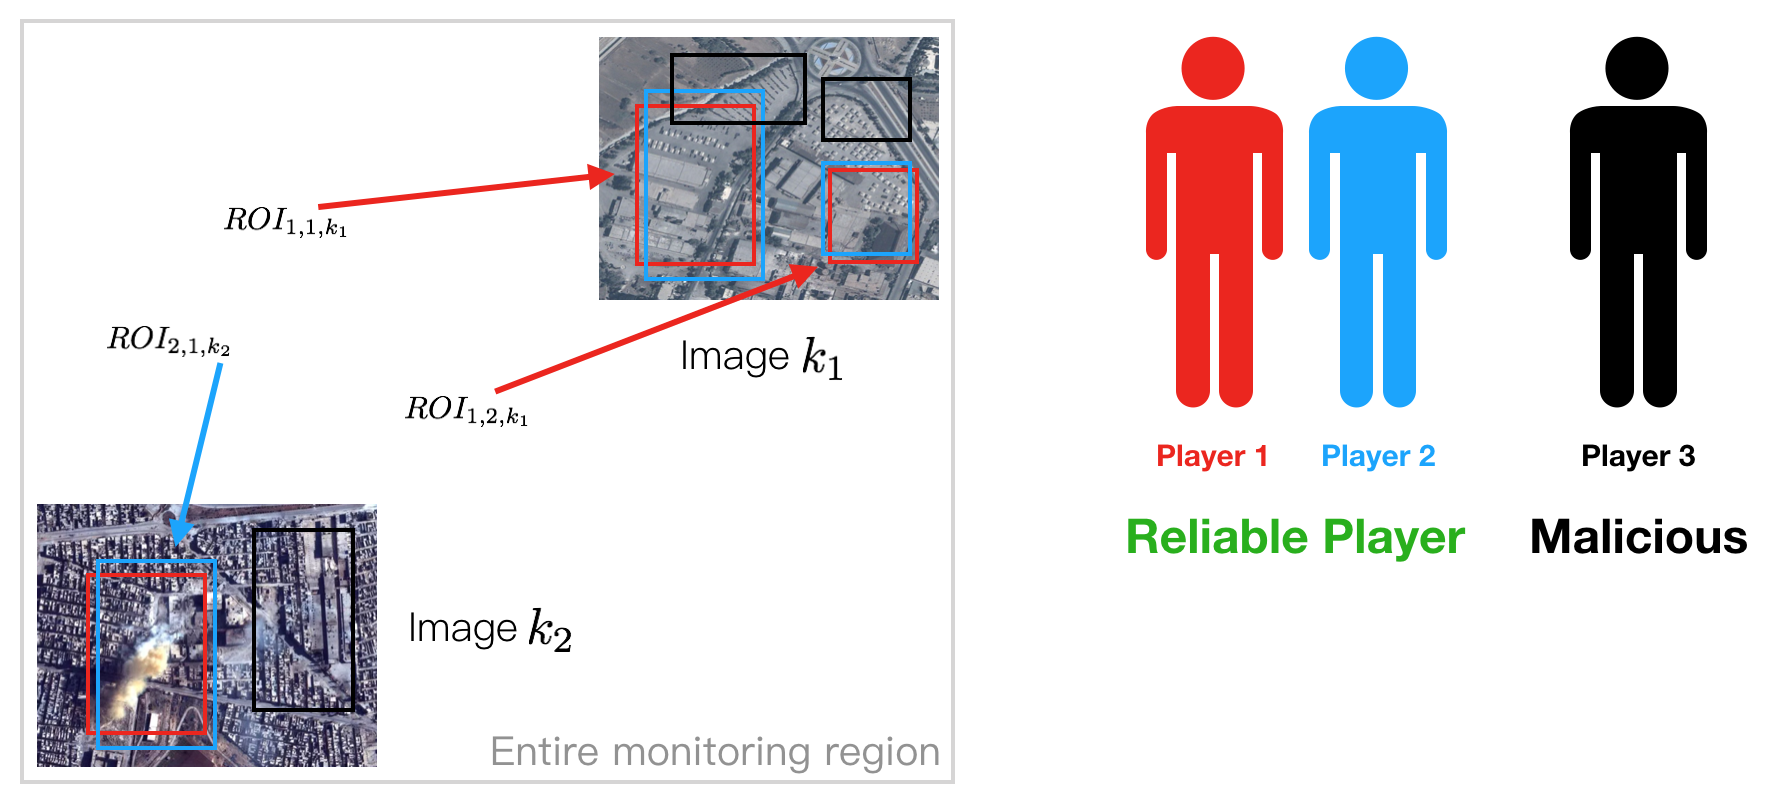
\includegraphics[width=0.9\textwidth]{figures/roi}
\caption{Examples of Region of Interests (ROI)}
\label{fig:roi}
\end{figure}

With this definition, our system players are able to select ROIs for each image as well as capable of select tags for each ROI.
Thus, the \emph{tasks} field in PlayerDB is an array object, stores each player image result with an assigned \emph{image\_id}.
Each object in the \emph{tasks} array has a field \emph{reliable}, which indicates the reliability for this object task;
Each object also contains a \emph{ROIs} field, which is an array object that contains the player inputs for this object image;
Each ROI object in the ROIs field has four properties that describes the ROI geometric location: \emph{x, y, height, width}, and 
also a \emph{tags} array field that describes the input tags for this image from this player.

For \emph{tags} field,
game players select the related tags for each ROI, and stores in this array. \textbf{Each tag can only selects once, 
and players allow to input their own new tags for this ROI.} Then, We define the ROI tag vector for the model design:

\begin{definition}
\label{def:tagv}
\emph{Assuming the database stores $n$ different tags $\text{tag}_1, \text{tag}_2, ..., \text{tag}_n$ for a certain image $k$,
the \textbf{Tag Vector} $T_{p, i, k}$ of $ROI_{p, i, k}$ (the $i$-th ROI in image $k$ of player $p$) is a vector that 
is donated by the following formula:}
\begin{equation}
  T_{p, i, k} = (|\text{tag}_1|, |\text{tag}_2|, ..., |\text{tag}_n|)
\end{equation}
\emph{where
\begin{itemize}
\item $\text{tag}_i$ is the $i$-th tag;
\item $n$ is the number of tags;
\item $|\text{tag}_i|$ is the count of $\text{tag}_i$ in a player task object.
\end{itemize}}
\end{definition}

Note that due to each tag can only selects once, the components of tag vector is \textbf{either 1 or 0} in reality.
For instance, for a certain image $k$,
there are 5 different tags $\text{tag}_1, \text{tag}_2, \text{tag}_3, \text{tag}_4, \text{tag}_5$ were inputed
by our game player.
Assuming player $p$ selects the first ROI and inputs tags for $ROI_{p, 1, k}$: 
$\{\text{tag}_1, \text{tag}_2, \text{tag}_3, \text{tag}_4\}$, 
player $q$ selects the first ROI and inputs tags for $ROI_{q, 1, k}$:
$\{\text{tag}_1, \text{tag}_3, \text{tag}_4, \text{tag}_5\}$. 
Then tag vector $T_{p, 1, k}$ of $ROI_{p, 1, k}$ is $(1, 1, 1, 1, 0)$ and tag vector
$T_{q, 1, k}$ of $ROI_{q, 1, k}$ is $(1, 0, 1, 1, 1)$.

\subsubsection{Player Task Generator}

The \textbf{\hyperref[idx:ptg]{PTG}} combines task images from satellite and ResultDB.
A player task contains $2n$ different images in random order, that $n$ images are
the untagged new satellite images and $n$ images are tagged images of ResultDB, which means
\hyperref[idx:ptg]{PTG} contains two generating steps:

\begin{itemize}
\item [Step 1.] \hyperref[idx:ptg]{PTG} shall split a monitoring region into small pieces of images, 
and also assign a unique \textbf{image\_id} for each piece 
(The reason is discussed in section \ref{chapter:ethical} for the leakage of data).

\item [Step 2.] \hyperref[idx:ptg]{PTG} shall retrieve tagged images from ResultDB. Then combine
all images as a user task assign to a new upcoming player.
\end{itemize}

\subsubsection{Player Rating Model}

This subsection describes the \textbf{\hyperref[idx:prm]{PRM}} as well as its detection algorithm 
inside our Disaster Monitoring system.
The \hyperref[idx:prm]{PRM} is responsible for detect malicious players regarding their game task inputs.

PageRank was first proposed by Lary Page \cite{page1999pagerank} and 
applied to social analysis in \cite{bonacich2001eigenvector}. 
It is commonly used for expressing the stability of physical systems and the relative importance, 
so-called \textbf{centralities}, of the nodes of a network. 
We transfer the basic idea of centralities of a network
and use eigenvalue as the trust value for each player to distinguish malicious players and reliable players.

We establish the model in image dependent perspective. For a certain image $k$,
considering a directed \textbf{Player Rating Graph (PRG)\label{idx:prg}} 
between players who tagged the image $k$. Each player is a node of PRG, 
as illustrated in figure \ref{fig:graph}. 

\begin{figure}[htp]
\centering
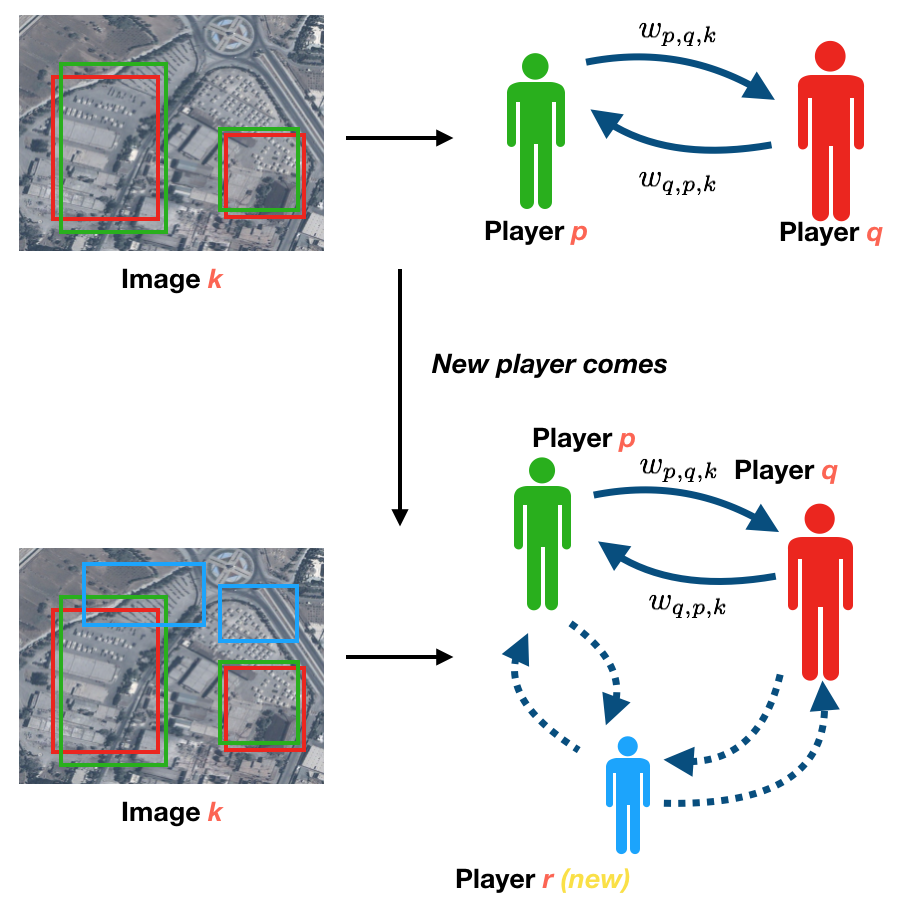
\includegraphics[width=0.5\columnwidth]{figures/graph2}
\caption{Player Rating Graph for Certain Images}
\label{fig:graph}
\end{figure}

\begin{definition}
\label{def:weightv}
\emph{
Assuming the database stores $n$ different tags $\text{tag}_1, \text{tag}_2, ..., \text{tag}_n$ in the system,
The \textbf{System Weight Vector} $v = (p(\text{tag}_1), p(\text{tag}_2), ..., p(\text{tag}_n))$ 
\textbf{of all tags} can be calculated by the following equation \ref{eq:ptag}:
\begin{equation}
\label{eq:ptag}
p(\text{tag}_i) = \frac{|\text{tag}_i|}{\sum_{j=1}^{n}{|\text{tag}_j|}}
\end{equation}
where  $|\text{tag}_i|$ is the count of $\text{tag}_i$ in the system.
}
\end{definition}
\begin{definition}
\label{def:weightvk}
\emph{
Assuming there are $r_s$ different tags $\text{tag}_{r_1}, \text{tag}_{r_2}, ..., \text{tag}_{r_s}$ were tagged in
a certain image $k$, the \textbf{Image Weight Vector} is a vector for image $k$ that is
composed by part of the System Weight Vector, which 
is donated by $v_k = (p(\text{tag}_{r_1}), p(\text{tag}_{r_2}), ..., p(\text{tag}_{r_s}))$
with $r_i (i=1,2,...,s) \in \{1, 2, ..., n\}$, $r_i \neq r_j (i\neq j, j=1,2,...,s)$ and $s \leq n$.
}
\end{definition}

For instance, the system have 2 different images. The first image is tagged by two players. One is 
$\text{tag}_1, \text{tag}_2, \text{tag}_5$ and another is $\text{tag}_1, \text{tag}_2$;
The second image is tagged by three players, their results are:
$\text{tag}_1, \text{tag}_2, \text{tag}_5$;
$\text{tag}_2, \text{tag}_4, \text{tag}_5$; 
$\text{tag}_3, \text{tag}_4, \text{tag}_5$. 
Thus, the system currently have 5 different tags $\text{tag}_1, \text{tag}_2, \text{tag}_3, \text{tag}_4, \text{tag}_5$.
Each tags ( $\text{tag}_1$ to $\text{tag}_5$) have corresponding counts: $3, 4, 1, 2, 4$; Therefore the
System Weight Vector is $(\frac{3}{14}, \frac{2}{7}, \frac{1}{14}, \frac{1}{7}, \frac{2}{7})$;
the Image Weight Vector of the first image is $(\frac{3}{14}, \frac{2}{7}, \frac{2}{7})$
since the first image only is tagged by $\text{tag}_1, \text{tag}_2, \text{tag}_5$, and
the Image Weight Vector of the second image is as same as the System Weight Vector
due to the second image is tagged by all exist tags.

Obviously, we have $0 \leq p(\text{tag}_i)\leq 1$, $\sum_{i=1}^{n}{p(\text{tag}_{i})}=1$ and $\sum_{i=1}^{s}{p(\text{tag}_{r_i})} \leq 1$.

To go so far as to this system, our player have two different type of inputs: \textbf{the \hyperref[def:roi]{ROI}, 
and its \hyperref[def:tagv]{Tag Vector}}. To define the \hyperref[idx:prg]{PRG} edge weight, 
we introduce two input measurements in the subsequent definition \ref{def:prmr} and \ref{def:pitc}.

\begin{definition}
\label{def:prmr}
\emph{
The \textbf{Players ROI Matching Ratio (PRMR)} is an importance measurement that measures the proportion of
two different \hyperref[def:roi]{ROI} intersection surface from player $p, q$ and 
the \hyperref[def:roi]{ROI} surface from player $p$ in a certain image $k$, 
which is donated by the following formula:
\begin{equation}
\text{PRMR}(p, q, i, j, k) = \frac{| ROI_{p,i,k} \cap ROI_{q,j,k} | }
       {|ROI_{p,i,k}|}
\end{equation}
where
\begin{itemize}
\item $ROI_{p, i, k}$ is the $i$-th selected ROI from player $p$;
\item $|ROI_{p, i, k}|$ is the surface of $ROI_{p, i, k}$;
\end{itemize}
}
\end{definition}

\begin{lemma}
\label{lemma:prmrrange}
\begin{equation}
\label{eq:prmrrange}
0 \leq \text{PRMR}(p, q, i, j, k) \leq 1
\end{equation}
\end{lemma}
\begin{proof}
According to the definition of \hyperref[def:roi]{ROI}, $| ROI_{p,i,k} \cap ROI_{q,j,k} |$ 
can archive its maximum value only and only if $ROI_{p,i,k} =  ROI_{q,j,k}$ 
as well as its minimum value only and only if $ROI_{p,i,k}$ has no intersection with $ROI_{q,j,k}$.
Thus:
\[
0 = \frac{0}{|ROI_{p,i,k}|} \leq \text{PRMR}(p, q, i, j, k) \leq
\frac{| ROI_{p,i,k} \cap ROI_{p,i,k} | }{|ROI_{p,i,k}|} = \frac{|ROI_{p,i,k}|}{|ROI_{p,i,k}|} = 1.
\]
\end{proof}

\begin{definition}
\label{def:pitc}
\emph{
The \textbf{Players Input Tag Correlation (PITC)} is an importance measurement that measures the proportion of
the covariance of two different \hyperref[def:tagv]{Tag Vector $T_{p,i,k}, T_{q,j,k}$} from player $p, q$ and the covariance of $T_{p,i,k}$ from player $p$ with itself under the
\hyperref[def:weightvk]{Image Weight Vector $v_k$}, which is donated by the following formula:
\begin{equation}
\text{PITC}(p, q, i, j, k) = \frac{Cov(T_{p,i,k}, T_{q,j,k}; v_k)}{Cov(T_{p,i,k}, T_{p,i,k}; v_k)}
\end{equation}
where $Cov(X, Y; w)$ is the weighted covariance between $X$ and $Y$, which donated by:
\begin{equation}
\label{eq:cov}
Cov(X, Y; w) = \frac{\sum_{i=1}^{n}{w_i(x_i-\frac{1}{n}\sum_{i=1}^{n}{w_i x_i})(y_i-\frac{1}{n}\sum_{i=1}^{n}{w_i y_i})}}{\sum_{i=1}^{n}{w_i}}
\end{equation}
with $X = (x_1, x_2, ..., x_n), Y = (y_1, y_2, ..., y_n), w = (w_1, w_2, ..., w_n)$.
}
\end{definition}

Note that

\begin{enumerate}
\item \textbf{The definition of PRMR and PITC share the same intent for measureing asymmetric importance  
      between player $p$ and player $q$ (how $p$ think of $q$)};
\item The definition of \textbf{PRMR is inspired by} a wide-used computer vision criteria, the so called \textbf{Intersection over Union (IoU)}, 
      also as known as \textbf{Jaccard Index} \cite{real1996probabilistic, wiki:JaccardIndex},
      which is a statistic used for comparing the similarity and diversity of sample sets. 
      However, in our case, we only divided by to guarantee the asymmetric property for directed graph weight;
\item The definition of \textbf{PITC is inspired by the Weighted Pearson Correlation Coefficient} \cite{wiki:PearsonCorrelationCoefficient},
      which is a measure of the linear correlation between two variables. In our case, with the same intent of PRMR, 
      we \textbf{drop} the
      part of covariance of player $q$ in denominator to guarantee the asymmetric property for directed graph weight; 
\item The PRMR and PITC both \textbf{are not metrics} due to $\text{PRMR}(p, q, i, j, k) \neq \text{PRMR}(q, p, i, j, k)$ as well as
$\text{PITC}(p, q, i, j, k) \neq \text{PITC}(q, p, i, j, k)$.
\end{enumerate}

\begin{lemma}
\label{lemma:pitcrange}
\begin{equation}
\label{eq:pitcrange}
-1 \leq \text{PITC}(p, q, i, j, k) \leq 1.
\end{equation}
\end{lemma}
\begin{proof}
We know that the weighted Pearson Correlation Coefficient \cite{wiki:PearsonCorrelationCoefficient} lies on $[-1, 1]$, i.e.
\[
  -1 \leq \frac{Cov(T_{p,i,k}, T_{q,j,k}; v_k)}{\sqrt{Cov(T_{p,i,k}, T_{p,i,k}; v_k)Cov(T_{q,j,k}, T_{q,j,k}; v_k)}} \leq 1
\]
To prove equation \ref{eq:pitcrange}, we have to show:
\begin{multline}
  \frac{Cov(T_{p,i,k}, T_{q,j,k}; v_k)}{Cov(T_{p,i,k}, T_{p,i,k}; v_k)} \\
  \leq |Cov(T_{q,j,k}, T_{q,j,k}; v_k)\sqrt{Cov(T_{p,i,k}, T_{p,i,k}; v_k)Cov(T_{q,j,k}, T_{q,j,k}; v_k)}| \leq 1
\end{multline}
and
\begin{multline}
  \frac{Cov(T_{p,i,k}, T_{q,j,k}; v_k)}{Cov(T_{p,i,k}, T_{p,i,k}; v_k)} \\
  \geq -|Cov(T_{q,j,k}, T_{q,j,k}; v_k)\sqrt{Cov(T_{p,i,k}, T_{p,i,k}; v_k)Cov(T_{q,j,k}, T_{q,j,k}; v_k)}| \geq -1
\end{multline}
Then we need to show:
\begin{equation}
0 \leq Cov(T_{p,i,k}, T_{p,i,k}; v_k)Cov(T_{q,j,k}, T_{q,j,k}; v_k)^3 \leq 1
\end{equation}
Considering $T_{p,i,k}, T_{q,i,k}$ are described in general, with equation \ref{eq:cov}, 
we only need to show (\textbf{$s$ is an vector components index} instead of exponential):
\begin{equation}
0 \leq Cov(T_{p,i,k}, T_{p,i,k}; v_k) = 
\frac{
  \sum_{s=1}^{n}{
    v_{k}^s
    \left(T_{p,i,k}^s - \frac{1}{n}\sum_{s=1}^{n}{v_{k}^s T_{p,i,k}^s}\right)^2
  }
}{
  \sum_{s=1}^{n}{v_{k}^s}
} \leq 1
\end{equation}
According to the definition of \hyperref[def:tagv]{Tag Vector} and \hyperref[def:weightvk]{Image Weight Vector},
the components of $T_{p,i,k}$ are either 1 or 0, 
the components of $v_k$ lies on $[0, 1]$, then we have:
\begin{equation}
0 \leq \left(T_{p,i,k}^s - \frac{1}{n}\sum_{s=1}^{n}{v_{k}^s T_{p,i,k}^s}\right)^2 \leq 1
\end{equation}
Therefore,
\begin{equation}
0 = \frac{
  \sum_{s=1}^{n}{
    v_{k}^s \cdot 0
  }
}{
  \sum_{s=1}^{n}{v_{k}^s}
} 
\leq Cov(T_{p,i,k}, T_{p,i,k}; v_k) \leq
\frac{
  \sum_{s=1}^{n}{
    v_{k}^s \cdot 1
  }
}{
  \sum_{s=1}^{n}{v_{k}^s}
} = 1
\end{equation}
which proves equation \ref{eq:pitcrange}.
\end{proof}

Thus far, we have enough techniques to define the edge weight of \hyperref[abbr:prg]{PRG}.
The definition is shown in definition \ref{def:edgeweight}.

\begin{definition}
\label{def:edgeweight}
\emph{
For a certain image $k$, the edge weight of the PRG from player $p$ to player $q$ is donated 
by the formula \ref{eq:weight}:
\begin{equation}
\label{eq:weight}
w_{p,q,k} = 
\sum_{j=1}^{n}{
\sum_{i=1}^{m}{ \left(
  \text{PRMR}(p, q, i, j, k)
  \left(
    \text{PITC}(p, q, i, j, k) + 2
  \right)
\right)}}
\end{equation}
with player $p$ selected $m$ ROIs, player $q$ selected $n$ ROIs.
}
\end{definition}

Our goal is to calculate the centrality of the nodes (players) of the network graph.
The \textbf{Perron Frobenius theorem} \cite{wiki:PerronFrobeniusTheorem} is a common knowledge that guarantees our goal
can be drift to the calculation of the adjacency matrix of \hyperref[abbr:prg]{PRG}.
In consequence, one can use the normalized adjacency matrix through the following formula \ref{eq:normalize}:

\begin{equation}
\label{eq:normalize}
A_k = (a_{p,q,k}) = (\frac{w_{p,q,k}}{\sum_{q}{w_{p,q,k}}})
\end{equation}

where $k$ is the image indicator.

\begin{theorem}
The normalized ajacency matrix $A_k$ of PRG of a certain image $k$ is irreducible, real, 
non-negative, column-stochastic, and diagonal element being positive.
\end{theorem}

\begin{proof}
\textbf{Irreducibility}: As shown in figure \ref{fig:graph}, for a certain image $k$, 
the \hyperref[abbr:prg]{PRG} is strong connected because the
player who selected ROIs in image $k$ has a direct connection to any other player who also selected ROIs in image $k$ 
(the edge weight is well defined according to equation \ref{eq:weight}).
Thus, since $A_k$ is an normalized strong connected PRG ajacency matrix, which proves $A_k$ is irreducible.

\textbf{Real elements}: With lemma \ref{lemma:prmrrange} and \ref{lemma:pitcrange}, each part of the equation \ref{eq:weight} 
are real number. Thus, of course, the matrix $A_k$ elements are calculated by equation \ref{eq:normalize} that are real elements.

\textbf{Non-negative elements}: With lemma \ref{lemma:prmrrange} and \ref{lemma:pitcrange}, we have:
\[
w_{p,q,k} = 
\sum_{j=1}^{n}{
\sum_{i=1}^{m}{ \left(
  \text{PRMR}(p, q, i, j, k)
  \left(
    \text{PITC}(p, q, i, j, k) + 2
  \right)
\right)}} 
\geq
\sum_{j=1}^{n}{
\sum_{i=1}^{m}{ \left(
  0 \cdot
  \left(
    -1 + 2
  \right)
\right)}} = 0
\]
that $w_{p,q,k}$ has its minimum value when $\text{PRMR}(p, q, i, j, k) = 0 (for all i=1,...,m; j=1,...,n)$ 
and $\text{PITC}(p, q, i, j, k) = -1 (\text{for all} i=1,...,m; j=1,...,n)$. Meanwhile,

\[
w_{p,q,k} = 
\sum_{j=1}^{n}{
\sum_{i=1}^{m}{ \left(
  \text{PRMR}(p, q, i, j, k)
  \left(
    \text{PITC}(p, q, i, j, k) + 2
  \right)
\right)}} 
\leq 
\sum_{j=1}^{n}{
\sum_{i=1}^{m}{ \left(
  1 \cdot
  \left(
    1 + 2
  \right)
\right)}} = 3mn
\]

that $w_{p,q,k}$ has its maximum value when $\text{PRMR}(p, q, i, j, k) = 1 (\text{for all} i=1,...,m; j=1,...,n)$ 
and $\text{PITC}(p, q, i, j, k) = 1 (\text{for all} i=1,...,m; j=1,...,n)$.
  
\textbf{Positive diagonal elements}: According to lemma \ref{lemma:pitcrange}, 
the diagonal elements can be formalized by follows:

\begin{equation}
\begin{aligned}
w_{p,p,k} &= 
\sum_{j=1}^{m}{
\sum_{i=1}^{m}{ 
  \left(
    \text{PRMR}(p, p, i, j, k)
    \left(
      \text{PITC}(p, p, i, j, k) + 2
    \right)
  \right)
}} \\
&\geq \sum_{j=1}^{m}{
\sum_{i=1}^{m}{ \left(
  \frac{| ROI_{p,i,k} \cap ROI_{p,j,k} | }{|ROI_{p,i,k}|}
  \left(
    -1 + 2
  \right)
\right)}} \\
&= \sum_{j=1}^{m}{
\sum_{i=1}^{m}{
  \frac{| ROI_{p,i,k} \cap ROI_{p,j,k} | }{|ROI_{p,i,k}|}
}}\\
&= \sum_{i=j}{\frac{| ROI_{p,i,k} \cap ROI_{p,j,k} | }{|ROI_{p,i,k}|}} 
 + \sum_{i\neq j}{\frac{| ROI_{p,i,k} \cap ROI_{p,j,k} | }{|ROI_{p,i,k}|}}\\
&\geq \sum_{i=j}{\frac{| ROI_{p,i,k} \cap ROI_{p,j,k} | }{|ROI_{p,i,k}|}}\\
&= \sum_{i=1}^{m}{\frac{| ROI_{p,i,k} \cap ROI_{p,i,k} | }{|ROI_{p,i,k}|}}\\
&= \sum_{i=1}^{m}{\frac{| ROI_{p,i,k}|}{|ROI_{p,i,k}|}}\\
&= m > 0
\end{aligned}
\end{equation}

\textbf{Column stochastic}: according to the definition of matrix $A$, the sum of the column
elements are:
\begin{equation}
  \sum_{q}{a_{p,q,k}} 
  = \sum_{q}{ \frac{w_{p,q,k}}{ \sum_{q}{w_{p,q,k}} }}
  = \frac{\sum_{q}{w_{p,q,k}}}{\sum_{q}{w_{p,q,k}}} = 1
\end{equation}
\end{proof}

We have proved the existence and uniqueness of eigenvalues of normalized PRG adjacency matrix; 
one can use the corresponding eigenvalues to represent the trust value of players. Thus, we have:

\begin{definition}
A \textbf{Trust Value} $TV_i$ of player $i$ represents by the $i$-th eigenvalue of normalized PRG ajacency matrix $A$.
\end{definition}

This definition can represent the rating score from $i$ to $j$. With the trust value of players,
we propose our classification algorithm:

\begin{algorithm}[H]
\label{algo:malicious}
\SetAlgoLined
\SetKwInOut{Input}{input}\SetKwInOut{Output}{output}
\Input{anonymous IDs, TVs}
\Output{(anonymous\_id, isReliable)}
Calculate $TV_{new}$ as the trust value of player $new$ \;
\eIf{$TV_{new} \geq \frac{1}{|\text{players}|}\sum_{i\in \text{players}}{TV_{i}}$}{
  return $(\text{anonymous\_id}, \text{true})$
}{
  return $(\text{anonymous\_id}, \text{false})$
}
\caption{Player Classification Algorithm}
\end{algorithm}

In this algorithm, the criterion of classifying new players performs the action that 
the trust value of a new player should not be less than the mean value of overall trust value of players, 
which means the tagging performance of new player should not worth than result performance of former players.

Terefore in short, the input and output Data Model of PRM are as follows. For input:\\
$(\text{anonymous\_id}, \text{area\_id}, \text{time}, \text{ROIs}, \text{tags})$; 
For model output: 
$(\text{anonymous\_id}, \text{TV})$.

\subsubsection{Disaster Evaluation Model}
\label{chapter:dem}

For an area at time $t$, we address the \textbf{Disaster Evaluation Model (DEM)} 
via disaster level definition as follows:

\begin{definition}
\label{def:dl}
The \textbf{Disaster Level (DL)} of a monitor region is calculated by each area components:
\[
  DL = \sum_{\text{area}\in\text{region}}{DL_{\text{area}}}
\]
where $DL_{\text{area}}$ is calculated by its corresponding tag vector:
\[
  DL_{\text{area}} = \sum_{i=1}^{n}{v_i \times |\text{tag}_i|}
\]
with $n$ is the number of current exist tags, and $|\text{tag}_i|$ is the occurrance of $\text{tag}_i$
in the corresponding area.
\end{definition}

System like ESP \cite{von2004labeling}, ARTigo \cite{wieser2013artigo} has proved that 
human inputs are valuable and useful.

Note that sometimes player carries new tags for our system, we also address a solution 
for this issue via the following steps:

\begin{itemize}
\item When a player carries predefined tags: Trivial;
\item When a player carries new tags: Directly drop, it is an unreliable result;
\item When a player carries predefined tags and also new tags: calculate the trust value without new tags;
  merge and update all weight vector $v$ via formula \ref{eq:weight} if the player is reliable, 
  otherwise drop and mark the result is unreliable.
\end{itemize}

With this definition \ref{def:dl}, we can calculate the disaster level for a monitoring region.
To sum up, the input and the output Data Model of DEM addresse as follows. For input:
$(\text{time})$, $(\text{area\_id})$ or $(\text{area\_id}, \text{time})$; For output:
$(\text{area\_id}, \text{time}, \text{disaster\_level})$.

\subsection{Model Initialization}
\label{chapter:modelinit}

A cold start of such a system is a common problem in human computation system that 
is avoided by hiring people to play or learn as long as 
the number of users or the quantity of data is insufficient.
In our system, we have two different cold start problem.

The first cold start problem appears in the PTG. To initialize the whole system, we need to
address an initial trusted group for PTG; they shall tagging enough initial trusted result
for PTG and then assign to new upcoming players. When a new player is reliable,
then the result of this player will become reliable. Meanwhile, the trusted group and 
available dataset grow larger with this step repeatedly, as shown in figure \ref{fig:cold}.

\begin{figure}[htp]
\centering
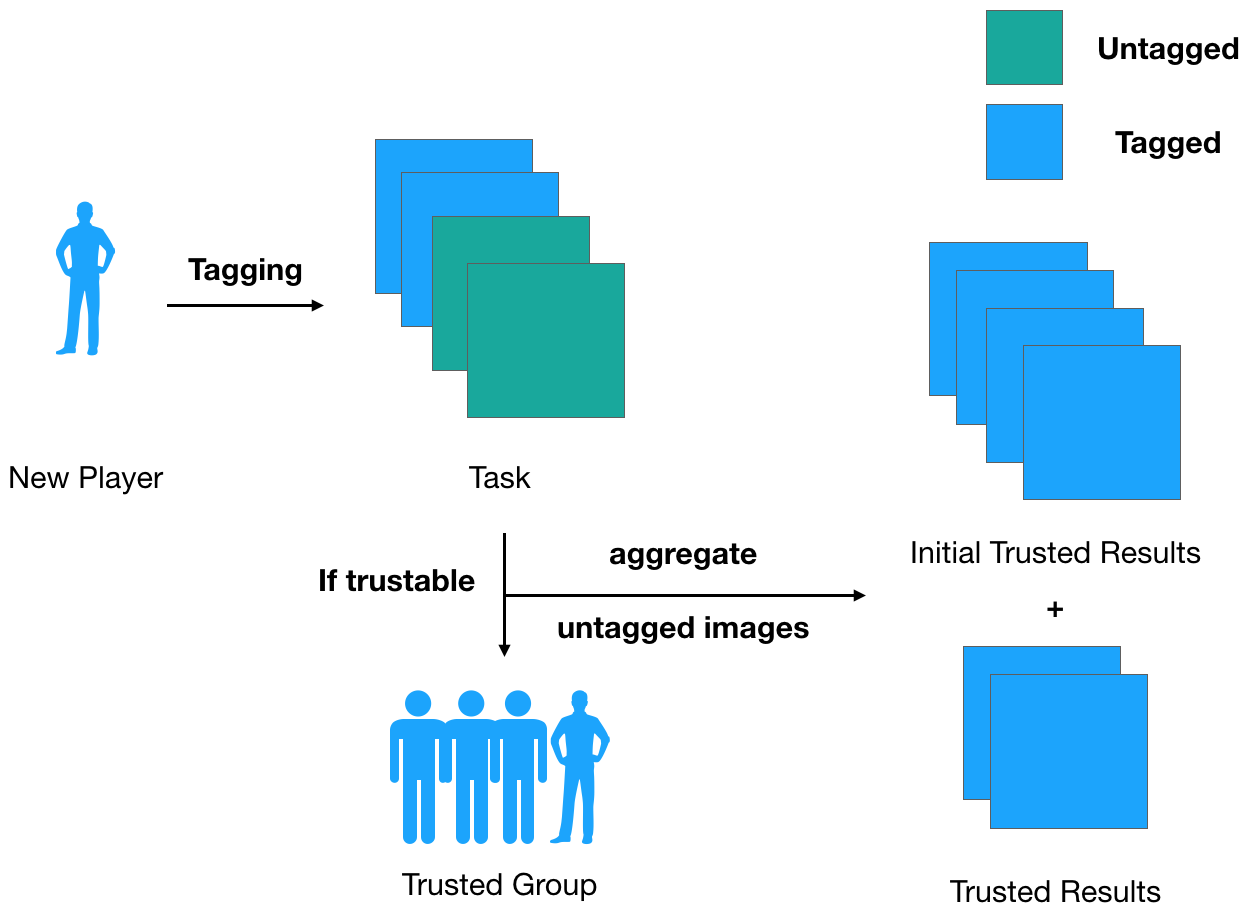
\includegraphics[width=0.5\columnwidth]{figures/coldstart}
\caption{Cold Start of PTG}
\label{fig:cold}
\end{figure}

The second cold start problem appears in PRM. According to the definition \ref{eq:weight} of PRG, the weight
of PRG was defined by the trust value of all players. Nevertheless, the initial trusted group has
no trust value. Thus we need an initial value for $TV$. Note that TV\_i is in between of 0 and 1, thus:

\[
TV_{i}^{\text{init}} = \frac{1}{|\text{players}^{\text{init}}|}
\]

with $|\text{players}^{init}|$ is the number of initial trusted group. 

\subsection{Discussion on Image Independent Model}

\section{System Evaluation and Success Criteria}

\subsection{Limitation of the System}
\subsection{Evaluation and success criteria}
  \subsubsection{Model Evaluation}
  \subsubsection{Issues on Social Aspects}
  \subsubsection{Issues on Ethical Aspects}
\section{Conclusions and Future Works}

\subsection{Conclusions}

% 在这份报告中,我们提出了一个全面的针对灾难监控的人肉计算系统,并详细讨论了它数学理论基础、所导致的问题和可能的解决方案。
% 纵观全文,我们在「introduction」一章中简述了基于GWAPs的人肉计算系统的基本动机,介绍了灾难监控存在的基本问题,
% 探讨了将人肉计算系统应用到灾难监控这个领域,作为人类一方的贡献应该如何设计。
In this report, we proposed a comprehensive design of a human computation system for disaster monitoring,
and we discussed its mathematical foundations as well as the possible issues caused by this system,
then gives few options to solve these issues. 

% 在「functionality」一章中,我们给出了一个提供给玩家和利益相关方的 GWAPs-based 的灾难监控的
% 人肉计算系统原形,并描述了它必备的功能及交互逻辑。
% 作为系统实现的思考,我们站在当前工业最高水平的技术栈的角度,探讨了实现这样一个系统所需涉及的技术栈,
% 以及选择这个技术栈的优势和缺点。
In the chapter of functionalities, we illustrated a prototype GWAPs-based disaster monitoring
human computation system for game players as well as stakeholders, and then described its
necessary functions and interaction logic. On thoughts of system implementation, we decided to implement 
this system on the web, probed the possible technology frameworks and pointed out the reason of our choices.

% 然后,我们详细描述了整个系统能够顺利并合理运行的全部理论细节,首先通过人工特征定义了一个用于计算玩家可信度的PRM,
% 描述了在这个模型下,对恶意用户进行检测判断的算法。作为 justification,我们给出了这个模型的合理性证明。
% 同时,作为聚合可靠用户输入数据的方法,我们给出了将灾难监控区域危险等级的计算转化为用户在监控图片上 tagging 任务的数学模型 DEM。
% 在这个模型中,我们使用站在贝叶斯观点下处理用户tagging的输入数据,防止了产生过多无用tag的问题。
% 当然,我们不可避免的需要处理这样一个人肉计算系统的「冷启动」初始化问题。
% 值得一提的是,在我们提出的系统设计下,启动整个系统理论上只需要非常小数量的可信用户组(两个人)即可。
Afterward, in the chapter of design, we modeled the entire system theoretically in details that make sure it can run consistently. First of all, we defined a \textbf{Player Rating Model}
for calculate a trust value of a player via artificial features, and then we put forward an algorithm
that can be used in malicious user detection. As justification, we proved the correctness of this model.
Meanwhile, as the data aggregation, we transferred the problem of calculating disaster level of regions into
processing the expectation value of user tagging task inputs and proposed the \textbf{Disaster Evaluation Model}.
In this model, we prevented the overabundance problem of potential useless tags from users by standing on the prespective of Bayesian. Surely, we addressed the solution of cold start of the human computation system.
It is worth mentioning that the minimum initial trusted group under this scheme design only requires two persons theoretically.

% 更进一步的,作为评估,我们首先给出了评价这个系统能够成功运行的的理论标准,然后陈述了这个系统在面临诸如数据安全、
% 信息泄露、恶意用户检测、用户匮乏以及xxx等问题时的挑战和解决手段。当然,这个目前这个系统还存在一些缺陷,
% 我们针对评估过期失效、信息丢失和游戏系统的可玩性三个问题进行了分析,并给出了可能的改进方案。
Furthermore, as evaluation, we discussed theoretical evaluation criteria for this system,
and then declared the challenges and corresponding solutions for facing issues like data security, information leakage, 
malicious detection as well as the lack of players.
Undoubtedly, the current system design still contains defects. Thus, we presented three analysis
and possible improvements for evaluation outdated, information loss and also gameplay playability. 

% 作为对进一步未来工作的思考,我们将在剩下的内容里简单讨论该系统一些可能的扩展形式、以及与其他人肉计算系统的交互。
For the future works, we will simply discuss the possible extension of our human computation system.

\subsection{Future Works}

Our system was described in general. We collect human inputs by ROI tagging tasks, 
which means any other HC system that related to ROI tagging tasks can easily use this system backend design.
In addition, due to the fact that we do not have enough user inputs at present, we use a certainty algorithm instead of 
uncertainty probablistic-based algorithm to detect malicious groups. 
Considering malicious detection is classification problem, which seperate users into trusted groups and untrusted groups. 
One can apply any classification machine learning algorithms that are more suitable for the detection of malicious groups 
if our user input dataset is large enough.

Besides, as we mentioned before, sometimes, the game player may encouter a situation that 
there is no ROI in some pictures which contain only landscapes like: mountains, rivers and forests.
In this case, with collaborative computing of image recoginition technique, we can filter out those images 
from our image database previously so that we can collect more data from the game and 
make our image tagging game more efficiently.

\section*{Acknowledgements}
\addcontentsline{toc}{section}{\protect\numberline{}Acknowledgements}
The authors would like to thank Prof. Fran\c{c}ois Bry first for
his great suggestions on information leak and loss problems of our disaster monitoring system;
we also thank Yingding Wang for his helpful discussions on system functionalities design 
and the model rationalization evaluation;
Finally, we also thank our schoolmate Huimin An for his inspiration of Bayesian perspective that
helps us handling human inputs with new tags successfully.

The resources of this project such as paper \LaTeX code, mockup drafts as well as
lab session beamer slides are open source on GitHub: \\
\url{https://github.com/changkun/hc-ss17-disaster-monitoring}.


\nocite{*}
\addcontentsline{toc}{section}{\protect\numberline{}References}
\bibliographystyle{ieeetr}
\bibliography{ref}
\end{document}
